%
%
% SUMMARY:
% USAGE:
%
% AUTHOR:       Christophe Prud'homme
% ORG:          Christophe Prud'homme
% E-MAIL:       prudhomm@zion
%
% ORIG-DATE:  7-Apr-04 at 16:48:32
% LAST-MOD:  7-Apr-04 at 23:07:19 by Christophe Prud'homme
%
% DESCRIPTION:
% DESCRIP-END.

\date{January 7 2008}

\begin{document}

% For every picture that defines or uses external nodes, you'll have
% to apply the 'remember picture' style. To avoid some typing, we'll
% apply the style to all pictures.
\tikzstyle{every picture}+=[remember picture]
\tikzstyle{na} = [baseline=-.5ex]

%By default all math in TikZ nodes are set in inline mode. Change this to
% displaystyle so that we don't get small fractions.
\everymath{\displaystyle}

\lecture[1]{Introduction}{intro}
\subtitle{Syllabus, History and Generalities}

\begin{frame}
  \maketitle
\end{frame}

\begin{frame}
  \tableofcontents
\end{frame}

\section{Organisation}

\subsection{Syllabus}
\begin{frame} \frametitle{Syllabus}
  \begin{tabular}[c]{lrl}
    Week   & Date  & \\\hline
    Week 2 & 7/01  & Course/TP\\
    Week 3 & 14/01 & Course/TP\\
    Week 4 & 21/01 & Course/TP\\
    Week 5 & 28/01 & Course/TP\\
    Week 6 & 04/02  & Course/Projects\\
    Week 7 & 11/02 & Course/Projects\\
    Week 8 & 18/02 & \alert{Vacations}\\
    Week 9 & 25/01 & Course/Projects\\
    Week 10 &03/03 & Course/Projects\\
  \end{tabular}
  \begin{block}{}
    \begin{itemize}
    \item 8 courses sessions (duration: 1.5h)
    \item 4 exercise sessions (duration: 1.5h)
    \item 4 homework/projects sessions (duration: 1.5h)
    \end{itemize}
    
  \end{block}

\end{frame}

\begin{frame} \frametitle{Schedule}
  \begin{itemize}
  \item Courses will be given in room 114 
  \item Exercises and Projects session will be done in room 212
  \end{itemize}
\end{frame}


\begin{frame} \frametitle{Final Grade}
  \begin{itemize}
  \item $N_p$ Project grade(about  10 minutes presentation and 10 minutes questions)
  \item $N_e$ Exam grade
  \item $N$ final grade
  \end{itemize}
  \begin{alertblock}{}
    \[ N = .5 N_p + .5 N_e + \mbox{ Bonus TP} \]
  \end{alertblock}


\end{frame}

\subsection[Notes]{Course Notes, TP and Projects}
\begin{frame}{Course Notes, TP and Projects}

  \begin{block}{}
    \begin{itemize}
     \item Course notes, TP and projects are available on the course website
       \begin{alertblock}{}
         \url{http://code.google.com/p/scicomp}
       \end{alertblock}
    \item Course notes will be distributed once the course has been given
    \item \alert{A correction for the TP will be given?}
    \item \alert{TP must be given back the day before the next course no later than midnight?}
    \end{itemize}
  \end{block}

\end{frame}

\begin{frame}{Project: Engineering design of a cooling system for CPUs}
  \begin{block}{}
    
  \end{block}
\end{frame}


\section[Objectives]{Scientific computing, what for ?}

\subsection[Focus]{Objectives}

\begin{frame}
  \frametitle{What is this course about ?}
  \begin{block}{Learning about}
    \begin{itemize}
    \item Numerical methods
    \item Scientific programming environments
      \begin{itemize}
      \item Compilers (C/C++)
      \item Paralell computing using MPI
      \item Scientific Libraries
      \item Programs for scientific computing
      \end{itemize}
    \item Scientific programming
    \item Pre and post processing
    \end{itemize}
  \end{block}
\end{frame}


\begin{frame}{Outline}
  \begin{itemize}
  \item Approximation and representation
  \item Root finding and integration
  \item Finite/hp spectral element method
  \item Linear Algebra
  \item Testing numerical codes (convergence rate, stability,
    dissipation, dispersion...)
  \end{itemize}
\end{frame}

\begin{frame}{Being practical}
  \begin{alertblock}{What if Scenarii}
    Imagine a situation where you don't have any commercial software
    to solve a given scientific computing problem:
    \centerline{What would you do ?}
  \end{alertblock}
\end{frame}

\begin{frame}<1-7>{What Would You Do?}
  \begin{block}{}

  \mode<presentation>{\begin{itemize}[<+-| alert@+>]}
  \mode<article>{\begin{itemize}}
  \item Ask the person that seem to know a lot about computing in your company
  \item Ask Google
  \item Ask other search engines
  \item Ask FOSS Community
  \item Ask your preferred GNU/Linux / FreeBSD distro  
  \item What else ?
  \end{itemize}
    
  \end{block}
  \only<7>{
    \begin{alertblock}{FOSS}
      We shall use FOSS
    \end{alertblock}
  }
\end{frame}

\begin{frame}{Numerical tools}
  \begin{itemize}
  \item Freefem++
  \item Python: numpy, scipy, pyx...
  \item Octave(aka Matlab free clone) and Octave toolboxes (Sourceforge)
  \item Look at free software db for scientific computing
  \end{itemize}

  \begin{block}{Issues}
    Understand mathematical software design and choices and
    programming techniques 
  \end{block}
\end{frame}


\begin{frame}[containsverbatim]{Why C++?}
  \begin{columns}
    \column{.5\textwidth}
    \begin{figure}[htbp]
      \centering
      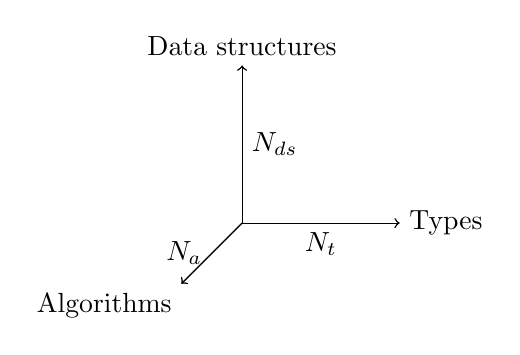
\begin{tikzpicture}[scale=2]
        \pgfsetarrowsend{to}
        \pgfpathmoveto{\pgfpointorigin}
        \pgfpathlineto{\pgfpointxyz{0}{0}{1}}
        \pgfusepath{stroke}
        \pgfpathmoveto{\pgfpointorigin}
        \pgfpathlineto{\pgfpointxyz{0}{1}{0}}
        \pgfusepath{stroke}
        \pgfpathmoveto{\pgfpointorigin}
        \pgfpathlineto{\pgfpointxyz{1}{0}{0}}
        \pgfusepath{stroke}
        \draw [->] (0,0) -- (1,0,0) node [right] {Types}; %%: \verb+int,double...+};
        \draw [->] (0,0) -- (0,1,0) node [above] {Data structures};
        \draw [->] (0,0) -- (0,0,1) node [below left] {Algorithms};

        \pgfsetarrowsend{}
        \draw (0.5,0,0) node [below] {$N_t$} (0,0,0.5) node [left] {$N_{a}$} (0,0.5,0) node [right] {$N_{ds}$};
      \end{tikzpicture}
      \caption{Components space of a program}
      \label{fig:1}
    \end{figure}

    \column{.5\textwidth}
  \begin{itemize}
  \item Basic algorithm support
    \begin{itemize}
    \item partitioning
    \item recursive function calls
    \item dynamic  memory allocation
    \item encapsulation
    \item templates
    \item ...
    \end{itemize}
  \item Support for multiple programming paradigms: OO, meta, functional,...
  \item Not only scientific computing but also many other application domains
  \end{itemize}
\end{columns}
\begin{alertblock}{Reduced program/library size}
  $N_t + N_{ds} + N_a$ instead of $N_t \times N_{ds} \times N_a$
  thanks to \lstinline+template+s and iterators (see STL)
\end{alertblock}
\end{frame}

\begin{frame}[containsverbatim]{Why MPI?}
  \begin{itemize}
  \item Message passing interface
  \item Natural and simple partitioning of problems
  \item Portability and efficiency
  \item Standard
  \end{itemize}
  \begin{block}{Remark on OpenMP}
    \begin{itemize}
    \item Distributed shared memory (Open MultiProcessing)
    \item Support for C/C++ and Fortran
    \item Multithread (multicore) but requires little invasive changes in the code (use of \lstinline+pragma+s)
    \item new paradigm MPI (inter-node)+OpenMP(intra-node) with nodes being multicore
    \end{itemize}
  \end{block}
\end{frame}
\subsection[Definition]{A definition of scientific computing}

\begin{frame}<1-2>{Scientific Computing: Definition}

      \only<1>{
        \begin{block}{What is Scientific Computing?}
        Can someone give a definition?
      \end{block}
      }
      \only<2>{
        \begin{block}{What is Scientific Computing?}
        Everything that is related to computing in science
      \end{block}        
      \begin{example}
        Geophysics, Astrophysics, Weather forecast, Global Change,
        Plasma physics, Aerodynamics, Hydrodynamics, MHD, Rheology,
        Materials processing, Molten metals, Finance 
      \end{example}
    }

\end{frame}

\begin{frame}{Scientific Computing: Position}

  \begin{block}{Position}
      How would you position Scientific Computing?
  \end{block}

\end{frame}

\begin{frame}
  \frametitle{Scientific Computing~(S.C.) = $\cap $\{Math.,Comp.Sci,Model.\}}
  \begin{columns}
    \begin{column}{.6\textwidth}
      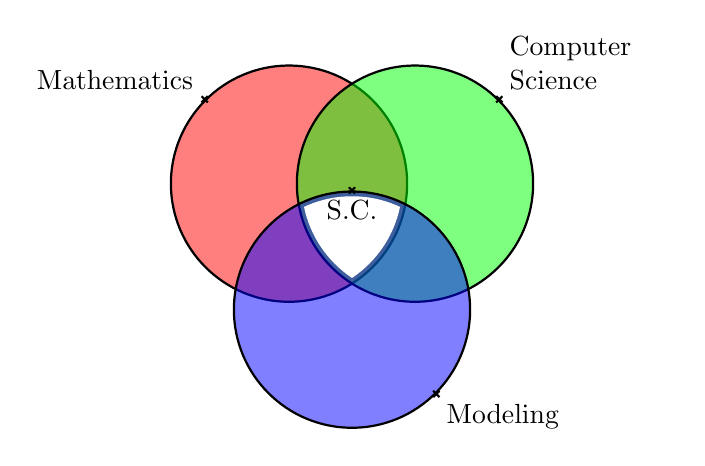
\begin{tikzpicture}[thick, scale=.8]
        \draw (0,2) node[fill=red,fill opacity=0.5,draw,shape=circle,name=cs,minimum size=3cm] {};
        \draw (2,2) node[fill=green,fill opacity=0.5,draw,shape=circle,name=math,minimum size=3cm] {};
        \draw (1,0) node[fill=blue,fill opacity=0.5,draw,shape=circle,name=model,minimum size=3cm] {};
        
         \begin{scope}{fill=white,fill opacity=1}
           \clip (0,2) circle (1.8cm);
           \clip (2,2) circle (1.8cm);
           \clip (1,0) circle (1.8cm);
           \fill[white] (1,0) circle (3cm);
         \end{scope}
         write label
         \draw[shift=(cs.north west)] plot[mark=x] coordinates{(0,0)} node[anchor=north east,text width=2cm,text ragged,above left] {Mathematics};
         \draw[shift=(math.north east)] plot[mark=x] coordinates{(0,0)} node[anchor=north west,text width=2cm,text ragged,above right] {Computer Science};
         \draw[shift=(model.south east)] plot[mark=x] coordinates{(0,0)} node[anchor=south west,text width=2cm,text ragged,below right] {Modeling};
         \draw[shift=(model.north)] plot[mark=x] coordinates{(0,0)} node[below] {S.C.};
      \end{tikzpicture}
    \end{column}
    \begin{column}{.4\textwidth}
      \begin{itemize}
      \item Primary objective:\\
        Mumerical experiments

      \item Secondary objective:\\
        \alert{How} to obtain them
        \begin{itemize}
        \item Mathematics
        \item Computer science/Software design
        \end{itemize}
      \end{itemize}
    \end{column}
  \end{columns}
  \begin{alertblock}{Richard Hamming}
    The purpose of computing is insight, not numbers
  \end{alertblock}
\end{frame}


\begin{frame}
  \frametitle{Domains of SC}

  \begin{block}{Some Domains}
  \begin{itemize}
  \item Military
  \item Basic research
  \item Industry
  \item Economy
  \item Life Sciences
  \end{itemize}
  \end{block}
\end{frame}


\begin{frame}
  \frametitle{Goals of SC}
  \begin{block}{Some Goals}
    \begin{itemize}
    \item Improvement of technological design (Airplanes, Cars, Ships)
    \item Improving security (Car crash simulations)
    \item Advanced methodologies (Molting, Burning)
    \item Understanding of physical phenomena (Big bang, Astrophysics)
    \item Design/interpretation of experiments (Plasma physics, High energy physics)
    \item More efficient production and higher quality (Tissue cutting)
    \item Forecasts (Weather, Bourse, Climate)
    \item Comparisons (Data base search, Web, Genomics, Proteomics)
    \item Recognition, detection (Image processing)
    \item Constant evaluation (business, statistics)
    \end{itemize}
  \end{block}

\end{frame}


\begin{frame}
  \frametitle{Numerical Simulation Cycle}

  \tikzstyle{root concept}+=[concept color=white!80]
  \tikzstyle{level 1 concept}+=[concept color=red!80, sibling angle=72]
  \tikzstyle{every annotation}=[fill=black!50,opacity=0.5,text=white,scale=.7]
  \begin{tikzpicture}[->]
     \path[mindmap,concept color=black!60,text=white]
     node[concept,scale=.7] {Numerical Simulation Cycle}
     %node[concept,scale=.7] {Scientific Computing}
     [clockwise from=0]
     %child[concept,scale=.6] { node[concept,scale=.7] (phys) {Physics Mechanics Biology Processing} }
     child[concept,scale=.6] { node[concept,scale=.7] (phys) {Modeling} }
     child[concept,scale=.6] { node[concept,scale=.7] (am) {Applied   Math.} }
     child[concept,scale=.6] { node[concept,scale=.7] (nm) {Numerical   Math.} }
     child[concept,scale=.6] { node[concept,scale=.7] (cs) {Computer Science} }
     child[concept,scale=.6] { node[concept,scale=.7] (va) {Validation} }
     ;
     \node [annotation,below] at (phys.south east)
     {
       \begin{itemize}
       \item Geophysics
       \item Astrophysics
       \item Weather forecast
       \item Global Change
       \item Plasma physics
       \item Aerodynamics
       \item Hydrodynamics
       \item MHD
       \item Rheology
       \item Materials processing
       \item Molten metals
       \item Finance
       \end{itemize}
     };
     \node [annotation,below] at (am.mid)
     {
       \begin{itemize}
       \item Statistics
       \item Functional Analysis
       \item Partial differential equations,
       \item Stochastic equations, etc.
       \end{itemize}
     };
     \node [annotation,below] at (nm.west)
    {
      \begin{itemize}
      \item Numerical Analysis:
        Convergence, Errors
      \item Approximation methods:
        Space/time discretization
        FD, FE, FV, spectral
        method, particle
        simulation
      \item Algorithms: complexity, accuracy
      \item Mesh Generation, CAD
      \item Direct / iterative solvers
      \end{itemize}
    };
    \node [annotation,above] at (cs.north)
    {
    \begin{itemize}
    \item Architecture: vector, parallel,  scalar, cluster.
    \item Systems, Compilers. Libraries
      \item Data management, Visualisation
      \item Parallelisation: MPI, OpenMP
      \item Optimisation, Parameterisation
      \end{itemize}
    };
    \node [annotation,above] at (va.north)
    {
      \begin{itemize}
      \item Interpretation of numerical experiment
      \item Comparison with experiment

      \item \alert{Correction of models}
      \end{itemize}
    }
    ;

    \begin{pgfonlayer}{background}
      \draw [concept connection]
      (phys) edge node[above,sloped]{Analyze} (am)
      (am) edge node[above,sloped]{Analyze} (nm)
      (nm) edge node[above,sloped]{Implement} (cs)
      (cs) edge node[above,sloped]{Run} (va)
      (va) edge node[above,sloped]{Correct} (phys);
     \end{pgfonlayer}

\end{tikzpicture}
\end{frame}


\section[History]{Scientific Computing History}
\subsection{Hardware}

\begin{frame}{Pioneers}
  \mode<presentation>{\vspace*{-.4cm}}
  \begin{table}[l]
    \centering
    \begin{tabular}[c]{clll}
      \rowcolor[gray]{1}
      1642	& Blaise Pascal	& Mechanical & 	Add, substract \\
      \rowcolor[gray]{1}
      & & & \tiny tax collection\\
      
      \rowcolor[gray]{.7}
      1820	& C. F. Gauss & Human &		Least square fits\\
      \rowcolor[gray]{.7}
      & & & \tiny geodesy\\
      
      \rowcolor[gray]{1}
      ~1850 & Charles Babbage & Difference  & Add, substract, \\
      \rowcolor[gray]{1}
      & & engine & multiply, divide\\
      \rowcolor[gray]{1}
      & Ada Lovelace &  Programmable    & 	\\
      
      \rowcolor[gray]{.7}
      ~1935 & Konrad Zuse	& EM relays		& Destroyed 1944 \\
      
      \rowcolor[gray]{1}
      1943	& Alan Turing &	Tubes, relays 	& Colossus \\
      \rowcolor[gray]{1}
      & & & \tiny code breaking computer \\
      
      \rowcolor[gray]{.7}
      1946	& Eckert/Mauchley &	Tubes, relays	& Eniac -> Univac\\
      
      \rowcolor[gray]{1}
      1948	& John von Neumann &	Tubes &		IAS  \\
      \rowcolor[gray]{1}
      & & & \tiny modern serial arch.\\
      
      \rowcolor[gray]{.7}
      1948	& Bardeen, Brattain, & &		Transistor \\
      \rowcolor[gray]{.7}
      & Shockley & & invention \\
      
      \rowcolor[gray]{1}
      1972	& Slotnick, Burroughs, & NASA	&	Illiac IV\\
      \rowcolor[gray]{1}
      & & &  \tiny array processor\\
      
      \rowcolor[gray]{.7}
      1975 &	Seymour Cray	& Cray 1&		Vector computer
    \end{tabular}
    \caption{A list of pionneers in scientific computing}
    \label{tab:1.1}
  \end{table}
\end{frame}
\begin{frame}{A vision for home computing}
  The figure~\ref{fig:1.1} gives a vision for home  computing: 
  \begin{columns}
    \column{.4\textwidth}
    \begin{figure}[htbp]
      \centering
      \mode<presentation>{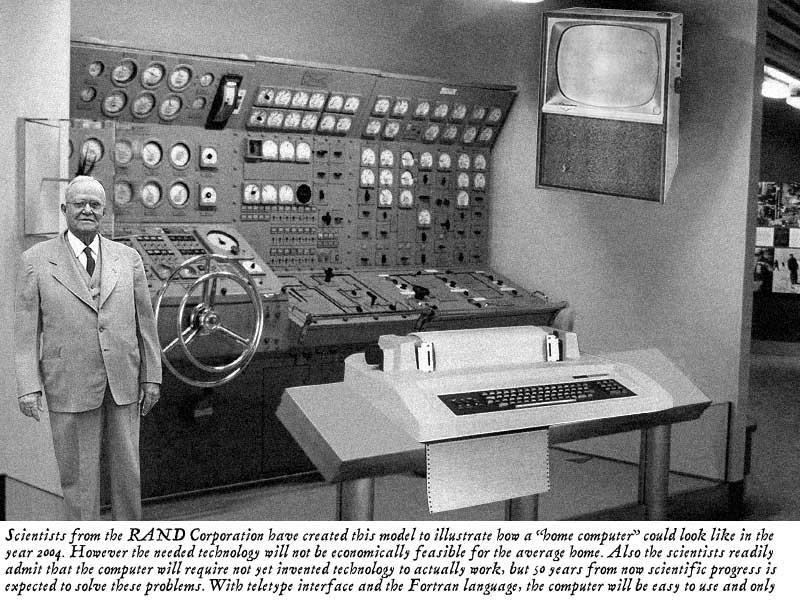
\includegraphics[width=1.2\textwidth]{computer_pioneer}}
      \mode<article>{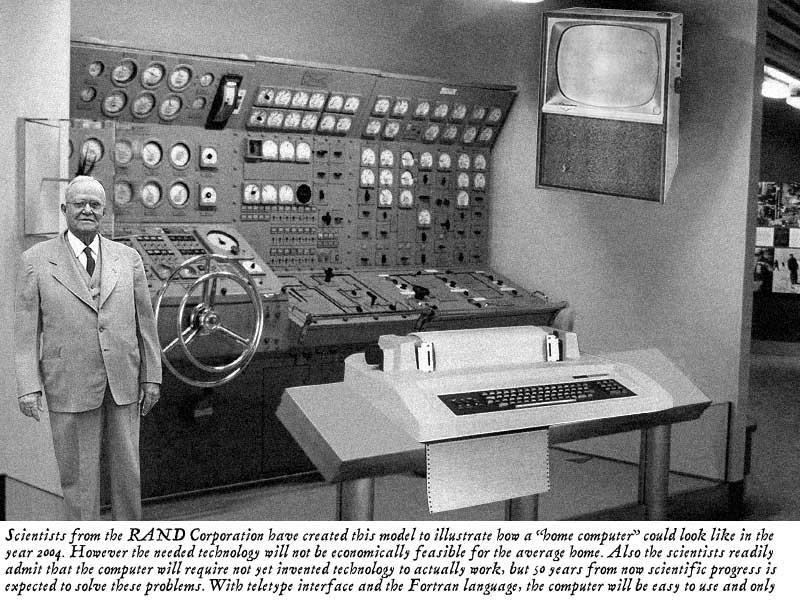
\includegraphics[width=\figwidth\textwidth]{computer_pioneer}}
      \caption{A vision for scientific computing}
      \label{fig:1.1}
    \end{figure}
    \column{.6\textwidth}
    \begin{quote}
      Scientists from the RAND Corporation have created this model to
      illustrate how a ``home computer'' could look like in the year
      2004. However the needed technology will not be economically
      feasible for the average home. Also the scientists readily admit
      that the computer will require not yet invented technology to
      actually work, but 50 years from now scientific progress is
      expected to solve these problems. With teletype interface and the
      Fortran language, the computer will be easy to use ...
    \end{quote}
  \end{columns}
\end{frame}

\begin{frame}{Computer Generations}
  \begin{table}[l]
    \centering

  \begin{tabular}{clll}
    
    \rowcolor[gray]{.7}
    First & 1945-54 & Vacuum tubes &	Mark 1, ENIAC, IAS,\\
    \rowcolor[gray]{.7}
    & & & IBM 701\\

    \rowcolor[gray]{1}
    Second &	1955-64 & Transistors	& CDC 1604, IBM 7000\\

    \rowcolor[gray]{.7}
    Third &	1965-74 & Integrated circuits &	CDC 6600\\

    \rowcolor[gray]{1}
    Fourth &	1975-90	& LSI/VLSI &		Cray 1, VAX 9000\\

    \rowcolor[gray]{.7}
    Fifth &	1991-now & ULSI/VHSIC &	Cray T3D, Intel Paragon\\
  \end{tabular}
    \caption{Computer generations table}
    \label{tab:1.2}
  \end{table}

\end{frame}

\subsection{Software }

\begin{frame}{Software History}
  
  \begin{table}[c]
    \centering
    %\rowcolors[]{1}{gray!70}{gray!100}
    \begin{tabular}[c]{lcl}
      \rowcolor[gray]{.7}
      Ada Lovelace	& 1850 &		Programmable difference scheme \\

      \rowcolor[gray]{1}
      Konrad Zuse		& 1945 &		Plankalk�l (algorithmic language)\\
      
      \rowcolor[gray]{.7}
      Grace Hopper	& 1954 &		Flowmatic (first compiler)\\

      \rowcolor[gray]{1}
      John Backus		& 1955 &		Fortran\\

      \rowcolor[gray]{.7}
      Bauer/Rutishauser	& 1958 &		Algol\\

      \rowcolor[gray]{1}
      Task Force		& 1959 &		Cobol\\
      
      \rowcolor[gray]{.7}
      K.E. Iverson	& 1962 &		APL (first parallel language)\\

      \rowcolor[gray]{1}
      D. Richie		& 1972 &		C\\

      \rowcolor[gray]{.7}
      Richie, Thompson	& 1978 &		Unix\\

      \rowcolor[gray]{1}
      Niklaus Wirth	& 1978 &		Modula-2 (OOP)\\

      \rowcolor[gray]{.7}
      J. Ichbiah		& 1979 &		ADA\\

      \rowcolor[gray]{1}
      B. Stroustrup	& 1983 &		C++\\

      \rowcolor[gray]{.7}
      Linus Thorvald	& 1992 &		Linux\\

      \rowcolor[gray]{1}
      V.S. Sundaram	& 1990 &		PVM\\
      
      \rowcolor[gray]{.7}
      MPI Forum		& 1995 &		MPI\\
      
      \rowcolor[gray]{1}
      Sun			& 1995 &		Java\\
    \end{tabular}
    \caption{Software history}
    \label{tab:1.3}
  \end{table}
  
\end{frame}
\subsection{Algorithms}
\begin{frame}{Algorithms History}
  \begin{tabular}[c]{lcl}
    \rowcolor[gray]{.7}
    Pythagoras, Thales	& -5th &		Geometry\\

    \rowcolor[gray]{1}
    Al-Khwarizmi	& 900 &		Algorithms\\

    \rowcolor[gray]{.7}
    Persia/Irak		& 1000 &		Algebra\\

    \rowcolor[gray]{1}
    Jobst B�rgi		& 1610 &		Logarithms\\

    \rowcolor[gray]{.7}
    John Napier		& 1614 &		Natural logarithms\\

    \rowcolor[gray]{1}
    J.B.J. Fourier	& 1808 &		Fourier Transform\\

    \rowcolor[gray]{.7}
    C.F. Gauss		& 1820 &		Gauss elimination/Least squares\\

    \rowcolor[gray]{1}
    C.G.J. Jacobi	& 1845 &		Jacobi method\\

    \rowcolor[gray]{.7}
    R. Courant		& 1943 &		Finite elements\\

    \rowcolor[gray]{1}
    Ulam, Metropolis	& 1946 &		Monte Carlo\\

    \rowcolor[gray]{.7}
    C. Lanczos		& 1950 &		Lanczos method\\

    \rowcolor[gray]{1}
    Stiefel, Hestenes	& 1952 &		Conjugate gradients\\

    \rowcolor[gray]{.7}
    H. Rutishauser	& 1958 &		LR/QR\\

    \rowcolor[gray]{1}
%    B.J. Alder		& 1959 &		Molecular dynamics\\

    
    G.B. Dantzig	& 1963 &		Linear programming\\

    \rowcolor[gray]{.7}
    Cooley, Tukey	& 1965 &		FFT\\

    \rowcolor[gray]{1}
    A. Brandt		& 1973 &		Multigrid\\
%    Car, Parinello	& 1985 &		Car Parinello method\\
  \end{tabular}
\end{frame}

\subsection[Quotes]{A Few Quotes}
\begin{frame}{A Few Quotes}
  \begin{block}{John von Neumann (Dec 28, 1903 - Feb 8, 1957)}
    It would appear that we have reached the limits of what it is
    possible to achieve with computer technology, although one should
    be careful with such statements, as they tend to sound pretty silly
    in 5 years. 
  \end{block}
\end{frame}

\begin{frame}{Quotes}
  \begin{block}{Edsger W. Dijkstra (1930-2002)}
%% When we had no computers, we had no programming problem
%% either. When we had a few computers, we had a mild programming
%% problem. Confronted with machines a million times as powerful, we
%% are faced with a gigantic programming problem.

    \begin{enumerate}
    \item  Besides a mathematical inclination, an exceptionally good mastery
      of one's native tongue is the most vital asset of a competent
      programmer.
      
    \item Programming is one of the most difficult branches of applied
      mathematics; the poorer mathematicians had better remain pure
      mathematicians.
      
    \end{enumerate}
    
  \end{block}
\end{frame}
%% Edsger W. Dijkstra (1930-2002) was a Dutch Computer Scientist,
%% invented the concept of "structured programming".
%%\end{frame}


\section[Programs]{Scientific Computing Programs}
\begin{frame}[label=scprog]
  \frametitle{What does a scientific program look like?}

  \tikzstyle{root concept}+=[concept color=gray!60]
  \tikzstyle{level 1 concept}+=[concept color=red!80, sibling angle=180]
  \tikzstyle{every annotation}=[fill=black!50,opacity=0.5,text=white,scale=.8]
  \begin{tikzpicture}[->]
    \path[mindmap,concept color=gray!70,text=white]
    node[concept,scale=.7] (proc) {Processing}
    % node[concept,scale=.7] {Scientific Computing}
    [clockwise from=0]
    % child[concept,scale=.6] { node[concept,scale=.7] (phys) {Physics Mechanics Biology Processing} }
    child[concept,scale=.7] { node[concept,scale=.7] (post) {Post Processing} }
    child[concept,scale=.7] { node[concept,scale=.7] (pre) {Pre Processing} }
    ;
    \node [annotation] at (proc.south)
    {
      \begin{itemize}
      \item Approximation methods: Space time discretisation, FE, FV,
        Particle methods,...
      \item Linear Algebra
      \end{itemize}
    };
    \node [annotation] at (pre.south)
    {
      \begin{itemize}
      \item Computer Aided Design (CAD)
      \item Mesh generation
      \end{itemize}
    };
    \node [annotation] at (post.south)
    {
      \begin{itemize}
      \item Interpretation of results
      \item Visualisation
      \end{itemize}
    };

    \begin{pgfonlayer}{background}
      \draw [concept connection,->]
      (pre) .. controls +(up:2cm) and +(up:2cm) .. node[above,sloped] {Data Handling} (proc)
      (proc) .. controls +(up:2cm) and +(up:2cm) .. node[above,sloped] {Data Handling} (post);
     \end{pgfonlayer}

  \end{tikzpicture}
\end{frame}

\subsection{Pre-Processing}

\begin{frame}
  \frametitle{Pre-Processing}
  \begin{block}{}
    \begin{itemize}
    \item CAD (OpenCascade)
    \item Mesh generation (gmsh, netgen, tetgen, ...)
    \item Data acquisition, properties(material...), ...
    \end{itemize}
  \end{block}
\end{frame}
\subsection{Processing}
\begin{frame}
  \frametitle{Processing: Algorithmic methodologies}
  \begin{block}{}
  \begin{itemize}
  \item Global functions approximations (FFT, wavelets, spectral methods)
  \item Local functions approximations (FE, FV, FD, p method)
  \item Monte Carlo simulations (MD, LB)
  \item Particle pushing (Gyrotron, Granular flow)
  \item Ray tracing (Image processing)
  \item Sequencing (Genomics, proteomics)
  \item Data handling (DB, Web)
  \end{itemize}
  
  \begin{itemize}
  \item Direct solvers
  \item Iterative solvers
  \item Time evolution (implicit, explicit)
  \item Eigenvalue problems
  \end{itemize}
  \end{block}
\end{frame}

\begin{frame}
  \frametitle{Processing: Parallel methods}
  \begin{block}{}
    \begin{itemize}
    \item Domain decomposition method
    \item Local parallelism (Point-to-point: FE, FV, FD, p-method)
    \item Global parallelism (All-to-many: FFT, wavelets, spectral)
    \item Redistribution/equilibration (Particle pushing)
    \item Embarassingly parallel applications (Master/slave: DB,
      Web, sequencing, ray tracing, parameter studies, statistics)
    \end{itemize}
  \end{block}
\end{frame}

\subsection{Post-Processing}
\begin{frame}{PostProcessing}
  \begin{block}{}
    \begin{itemize}
    \item Visualisation (Paraview, Octave, Pyx, Matplotlib,...)
    \item Analysis, validation
    \item Archive (HDF5,...)
    \item Error estimation, Adaptation, go back to preprocessing
    \end{itemize}
  \end{block}
\end{frame}


\subsection[Software]{Sofware Aspects}
\begin{frame}
  \frametitle{Software aspects}
  \begin{block}{A few things to consider}
    \begin{itemize}
    \item Control if results are correct: Bugs, not applicable models
    \item Improve precision: Single/double, stability (CFL), h,p,r methods
    \item Numerical experiments: Validation of models, interpretation of results
    \item Choose stable methods
    \item Convergence properties
    \item Portability, extensibility
    \item Efficiency, scalability, choice of adequate machine
    \item Engineering time: Production cycle, GUI
    \item Implementation aspects
    \end{itemize}
  \end{block}
\end{frame}



\begin{frame}
  \frametitle{Some words of wisdom?}
  \begin{block}{Machines}
    \begin{itemize}
    \item Use best single processor algorithms
    \item Parallelise, but only if single processor version is too slow/small
    \end{itemize}
  \end{block}
  \begin{block}{Applications/algorithms}
    \begin{itemize}
    \item Use what exists
    \item Use libraries, since they are efficiently implemented
    \end{itemize}
  \end{block}
\end{frame}





\end{document}

%%% Local Variables: 
%%% mode: latex
%%% TeX-master: t
%%% TeX-PDF-mode: t
%%% TeX-parse-self: t
%%% x-symbol-8bits: nil
%%% TeX-auto-regexp-list: TeX-auto-full-regexp-list
%%% ispell-local-dictionary: "american"
%%% End: 

